\begin{frame}{}

  \setlength{\parindent}{0pt}

  \vspace{-0.2cm}
  %% \begin{tabular}{ | p{0.44\textwidth}  | p{0.001\textwidth} | p{0.44\textwidth} |}
      \begin{tabular}{  p{0.43\textwidth}   p{0.02\textwidth}  p{0.43\textwidth} }

    \begin{center}
      \underline{\textit{\textbf{Standard random network model}}}    \end{center}

    &&

    \begin{center}
      \underline{\textit{\textbf{Varying connection probabilities}}}
    \end{center}

    \\

    \begin{center}\vspace{-0.71cm}
      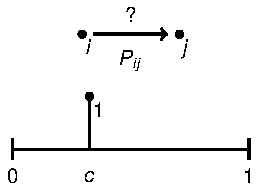
\includegraphics[width=0.69\linewidth]{%
        figures/tikz_line.pdf} %
    \end{center}%\vspace{1cm}

    &&

    \begin{center}\vspace{-0.71cm}
      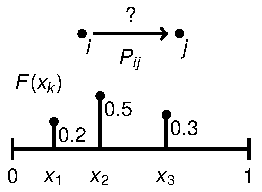
\includegraphics[width=0.69\linewidth]{%
        figures/tikz_line_right.pdf} % 
    \end{center}%\vspace{1cm}

    \\

    Probability of connection a \ul{constant} $P_{ij}$,
    %\vspace{0.05cm}
    
    \begin{align*}
      P_{ij} = c
    \end{align*}

    &&

    Probability of connection a \ul{random variable} $P_{ij}$,
    \vspace{0.01cm}
    
    \begin{align*}
      \mathbf{Prob}(P_{ij}=x_k) = F(x_k)
    \end{align*}	

    \\
    
    \textbf{Overall connection probability}
    \vspace{0.12cm}
    
    \begin{align*}
      \mu = P_{ij} = c
    \end{align*}


    &&

    \textbf{Overall connection probability}
    \vspace{-0.08cm}
    
    \begin{align*}
      \mu = \sum_{k=1}^m F(x_k) x_k
    \end{align*}
    
    \\

    \textbf{Bidirectional connection}
    \vspace{0.12cm}
    
    \begin{align*}
      P_{\text{bidir}} = P_{ij} P_{ji} = c^2
    \end{align*}	

    &&

    \textbf{Bidirectional connection}
    \vspace{-0.08cm}
    
    \begin{align*}
      P_{\text{bidir}} = \sum_{k=1}^m \sum_{l=1}^m F(x_k) x_k F(x_l | x_k) x_l %\label{eq:TT}
    \end{align*}	
    
  \end{tabular}


  
\end{frame}



\begin{frame}{}
  Assume that connection probabilities within pairs are identical,
  
\begin{align*}
  F(x_l | x_k) = \begin{cases} 1 & \text{if $l = k$} \\ 0 & \text{otherwise.} \end{cases}
\end{align*}
Then

\begin{align*}
  P_{\text{bidir}} = \sum_{k=1}^m \sum_{l=1}^m F(x_k) x_k F(x_l | x_k) x_l = \sum_{k=1}^m F(x_k) x_k^2 .
\end{align*}

\vspace{0.4cm}

\textit{Relative overrepresentation} $\varrho$ is the fraction

\begin{align*}
  \varrho = \frac{P_{\text{bidir}}}{\mu^2} = \frac{\sum_{k=1}^m F(x_k) x_k^2 }{\left(\sum_{k=1}^m F(x_k) x_k\right)^2}.
\end{align*}
By Jensen's inequality,

\begin{align*}
  \left(\sum_{k=1}^m F(x_k) x_k\right)^2 \leq \sum_{k=1}^m F(x_k) x_k^2  \quad \text{and thus} \quad \varrho \geq 1.
\end{align*}	
%% If and only if $m > 1$, that is when the probability distribution of connection probabilities is non-degenerate, strict inequality in (2) holds.  

\source{\normalsize \cite{Hoffmann2017}}
\end{frame}
